\section{Brainstorm}
\label{brainstorm}

A brainstorm session was organised with key stakeholders to discuss the initial concept.
The stakeholders were spread over the different potential end-users: researcher, principal investigator, data manager, research committee.
The goal of this session was to evaluate the initial concept, which is described in the previous section, and to find any `hidden' functions that were not apparent during the observations.

\paragraph{The execution}
Brainstorming is not an exact science, therefore there is no pre-defined schema to follow.
However, there are a lot of gurus describing guidelines to manage sessions.
The following list is an implementation of guidelines taken from Tyner Blain \cite{brainstormWebsite}:

\begin{enumerate}
	\item \textbf{Rules -} Make sure everyone is on the same level and understands what the point of the meeting is through a small introduction talk.
	\item \textbf{Time limit -} Guidelines describe short sessions, but due to the complexity of the system two sessions of one hour each were necessary.
		Step 3 (seed) was repeated in the second session to refresh the idea of the system for everyone.
	\item \textbf{Starting point -} In this case the initial concept described in section \ref{process-analysis} was used as a starting point.
		During the session big (A2) pieces of paper were used on which the seed's functions are written down. Figure \ref{fig:brainstorm-before} is a stylised version of the used paper schema.
	\item \textbf{Ideas -} The sessions are structured by the paper schema, each of the functions is discussed.
		Ideas for new functionality or differences are shortly (vocally) summarised by the session leader (in this case the researcher) and written on the same paper.
	\item \textbf{Prioritise -} For this step the guidelines are disregarded and prioritisation is based on group agreement.
		Three levels are used: must have, should have, nice to have.
		Any functions that are deemed unnecessary were already removed from the schema during the `ideas' step.
\end{enumerate}

\paragraph{Results: differences}
Outcomes of the brainstorm showed that many requirements were hidden when the initial concept was defined.
The revised complete research life cycle for the \project{} is:
\begin{itemize}
	\item researcher submits a data request;
	\item committee members check this request and either approve it or not;
	\item the system creates a subset of data which the researcher can access;
	\item after completion of the research the researcher uploads his/her paper;
	\item the committee members check this paper and either approves it or not;
	\item during the whole cycle the data manager keeps an overview of this process.
\end{itemize}

This whole cycle is to be supported by the \ivfsystem{}.
There are a couple of differences with the initial concept.
The first being that researchers should be allowed to register themselves into the system with a limited account (\ie{} no access to data, no data requests).
After registering, the data manager is responsible for approving their account.

Then the second difference shows, namely, the data request approval process will also reside in the system.
As said before, a request is a document which contains information the research committee needs to base their decision on.
This information in the case of the \ivfsystem{} is: research question, hypothesis, problem background, description of perceived methods to solve question, and the requested data.
The document is formulated by the researcher and after submission, managed by research committee members (\ie{} evaluated, voted on).

After the researcher has access to his/her data the next difference become apparent.
The stakeholders representing the researchers said that analysis will mostly be done offline.
They are known and comfortable with the software they are using and are unwilling to switch.

This brings us to the next difference, data is not to be downloaded over the internet due to privacy reasons. 
Access should be restricted such that only certain (physical) places have direct access to the \projectdata{}.
However, metadata such as a data dictionary (\ie{} a document describing what data is available in the repository) can be accessed over the internet.
This helps the researcher in formulating their data request and provides more opportunity for data reuse (\eg{} someone might be unwilling to travel long distances just to submit a request).

The last step in the research life cycle, the publication, should also be supported in the system.
Publications have to be approved by the research committee before they can be published.
As with the data request process, the researcher creates a document (\ie{} upload a paper to the system) which is evaluated and approved by the committee.

Lastly, two notable differences outside of the research life cycle.
No third parties should be allowed on the system, for now the data is too valuable and studying exactly what information can be passed on is not a priority.
Secondly, no unlinked data will be stored or used in the system.
It might be interesting to find correlations between linked and unlinked data, but that is not the goal of the \project{}.

The focus of the system switches from purely data support to also supporting other research related tasks.
This is clearly visible in the revised workflow, figure \ref{fig:research-workflow-after}, which shows that the balance has shifted from just the `Data' group to a much broader perspective.

\begin{figure}[hb]
	\centering
	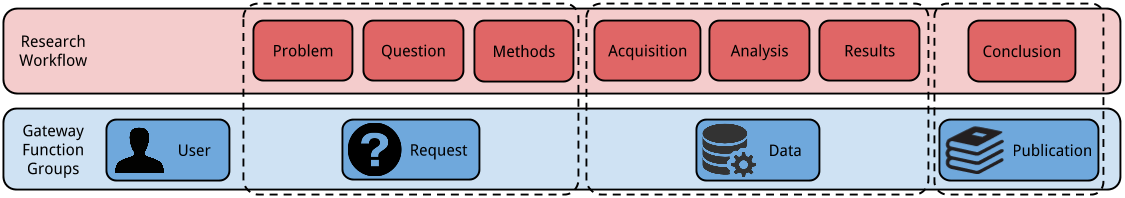
\includegraphics[width=1.0\linewidth]{images/research-workflow-after}
	\caption{
		Research workflow mapped by identified function groups after brainstorm, initial workflow shown in figure \ref{fig:research-workflow}.
		The user group underlays the whole system and is therefore outside of the dotted mapping lines.
	}
	\label{fig:research-workflow-after}
\end{figure}